% ============================================================================
% SEC02.TEX - Section 3.2: Lifecycle Functions
% ============================================================================

\section{Lifecycle Functions}

\begin{learningoutcomes}
\item Memahami urutan eksekusi lifecycle functions
\item Menggunakan Start(), Update(), Awake(), OnEnable()
\item Memahami kapan menggunakan setiap fungsi
\item Membedakan FixedUpdate() dan Update()
\end{learningoutcomes}

\subsection{Urutan Lifecycle Functions}

\begin{figure}[ht]
    \centering
    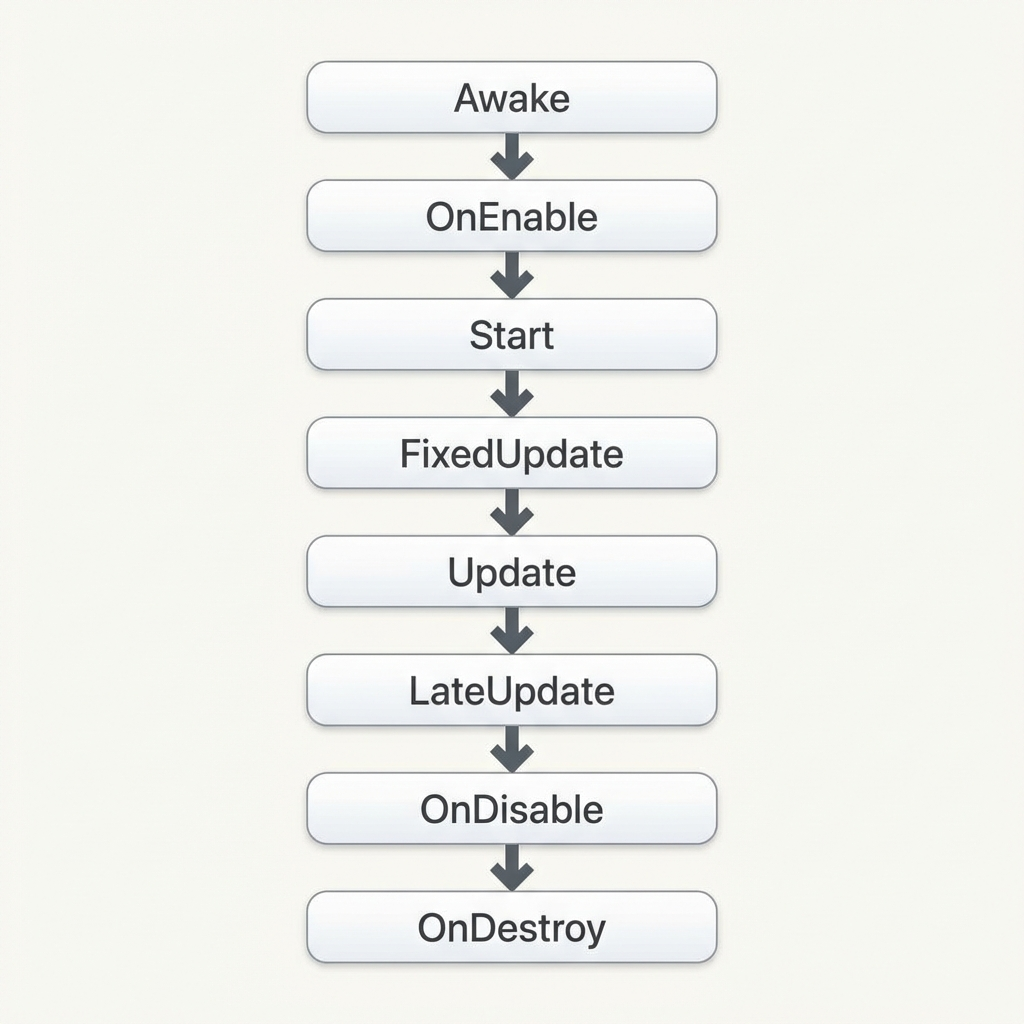
\includegraphics[width=0.6\textwidth]{figures/monobehaviour_lifecycle.png}
    \caption{Diagram Siklus Hidup MonoBehaviour}
    \label{fig:lifecycle}
\end{figure}

\begin{enumerate}
    \item \textbf{Awake()}: Dipanggil sekali saat object dibuat, sebelum Start()
    \item \textbf{OnEnable()}: Dipanggil setiap kali object diaktifkan
    \item \textbf{Start()}: Dipanggil sekali sebelum frame pertama Update()
    \item \textbf{Update()}: Dipanggil setiap frame (logika game)
    \item \textbf{FixedUpdate()}: Dipanggil pada fixed timestep (fisika)
    \item \textbf{LateUpdate()}: Dipanggil setelah semua Update() selesai (kamera)
    \item \textbf{OnDisable()}: Dipanggil saat object dinonaktifkan
    \item \textbf{OnDestroy()}: Dipanggil saat object dihancurkan
\end{enumerate}

\subsection{Contoh Implementasi}

\begin{lstlisting}[language={[Sharp]C}, caption=Contoh Lifecycle Functions]
using UnityEngine;

public class LifecycleExample : MonoBehaviour
{
    void Awake()
    {
        Debug.Log("Awake called");
    }
    
    void OnEnable()
    {
        Debug.Log("OnEnable called");
    }
    
    void Start()
    {
        Debug.Log("Start called");
    }
    
    void Update()
    {
        // Dipanggil setiap frame
    }
    
    void FixedUpdate()
    {
        // Dipanggil untuk fisika (default: 50x/detik)
    }
    
    void LateUpdate()
    {
        // Dipanggil setelah semua Update()
    }
    
    void OnDisable()
    {
        Debug.Log("OnDisable called");
    }
    
    void OnDestroy()
    {
        Debug.Log("OnDestroy called");
    }
}
\end{lstlisting}

\begin{catatan}
Gunakan Awake() untuk inisialisasi yang tidak bergantung pada GameObject lain. Gunakan Start() untuk inisialisasi yang memerlukan GameObject lain sudah siap.
\end{catatan}
